\begin{comment}
\documentclass[12pt,a4paper]{article}
\usepackage{a4wide}
\usepackage{amsfonts, amsmath, amsthm}
\usepackage[english]{babel}
\usepackage{framed}
\usepackage[pdftex]{graphicx}
\usepackage{epstopdf}
\usepackage[font=small,format=plain,labelfont=bf,up,textfont=it,up]{caption}
\usepackage{wrapfig}
\usepackage{tocloft}
\usepackage{psfrag}
\usepackage{subfig}
\usepackage[latin1]{inputenc}
\usepackage{verbatim}

%\usepackage{bbold}
\usepackage{bbm}
\topmargin -15mm
\textwidth 16truecm
\textheight 24truecm
\setlength\parindent{0pt}
\setlength\parskip{0.20in plus0.05in minus0.05in}
\newcommand{\Z}{\mathbb{Z}}
\newcommand{\N}{\mathbb{N}}
\newcommand{\R}{\mathbb{R}}
\newcommand{\C}{\mathbb{C}}
\newcommand{\eps}{\varepsilon}
\fboxrule 1pt
\fboxsep 7pt
\pagenumbering{arabic}
%3. In situ measuments of the reflection coefficient

%3.1 Adrienne method
%General intro, definition of reflection coeff
%Problems: directivity, no speakerdeconvolution

%3.2 Our method
%3 meters between mic and speaker
%3,15 meters high, not practical
%Helmholtz resonator

%3.3 Mls vs sweep
%mls16x64 - mls18x16 - sweep1X64 - sweep60

%3.4 Diffraction
%Measurement on the side of the wall?

%3.5 Our results vs Adrienne?

\begin{document}
\end{comment}


\section{In situ measurements of the reflection coefficient}
One of the objectives of our project was to develop a program in Matlab to record and process several acoustic signals to determine the sound characteristics of a wall. 
This section contains a description of our method; an assessment of the standard measuring method (the Adrienne method) and the results of an in situ measurement. 

\subsection{Recording method}
The particulars regarding the measurement equipment will be discussed in the following section; as well as the methods of data gathering and processing. Furthermore, a short description of the excitation signals will be given and finally the developed method will be put to the test by measuring the absorption characteristics of a Helmholtz resonator.

\subsubsection{Recording equipment}
% Weet niet goed wat er hier allemaal moet staan
The following hardware was used during the experiments:
\vspace{-20pt}
\begin{itemize}
	\setlength{\itemsep}{1pt}
  \setlength{\parskip}{0pt}
  \setlength{\parsep}{0pt}
	\item Octa-Capture sound card by Roland.
	\item Amplifier.
	\item Zircon loudspeaker.
	\item 1/2" Condenser Microphone Cartridge Type 4130 with Microphone Preamplifier Type 2642.
\end{itemize}

The software necessary to play and record sounds with these instruments was written in Matlab using the Data Acquisition Toolbox. The subsequent processing of these signals was also done in Matlab. The general content of this software will be discussed in section \ref{processing}. But in order to do accurate measurements, the specifics of the speaker have to be examined.

The impulse and frequency response of the Zircon speaker are shown in figure \ref{fig: ZirconImp}. The impulse response is rather short (less than 4 ms) and the frequency response has a smooth magnitude. To determine these responses, the measurement was performed in front of the speaker.
\begin{figure}[h!]
  \centering
    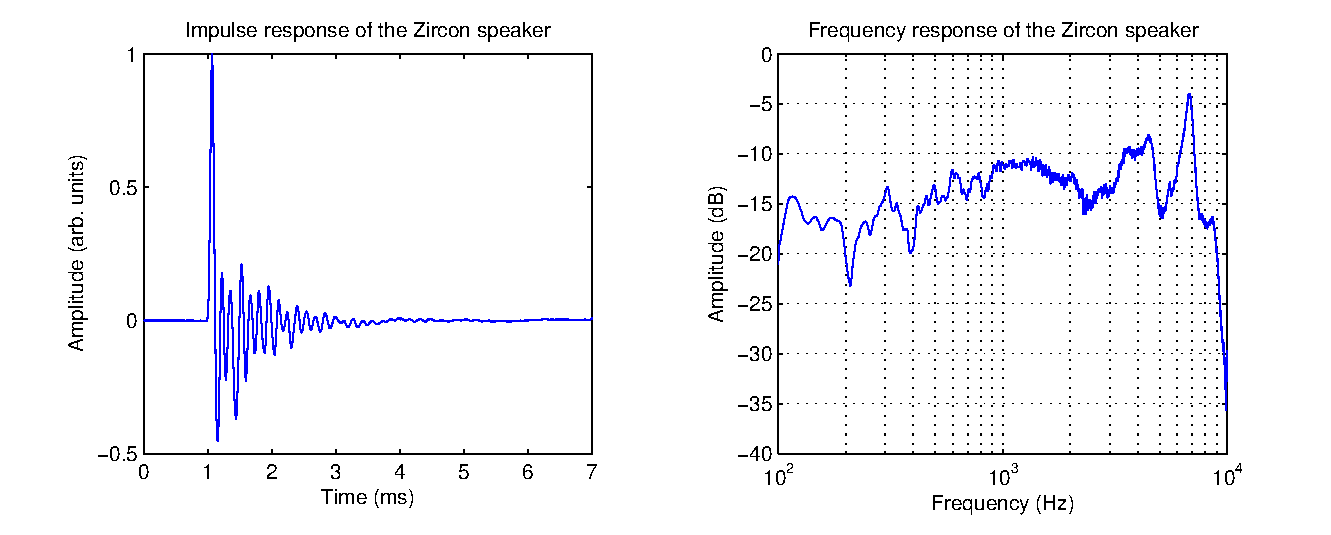
\includegraphics[width=\textwidth]{ZirconImpulse}
  %\vspace{-10pt}
  \caption{Impulse response and magnitude of the frequency response of the Zircon loudspeaker. The measurement was done in front of the speaker. }
  \label{fig: ZirconImp}
  %\vspace{-30pt}
\end{figure}



\begin{wrapfigure}{r}{0.2\textwidth}
	\vspace{-20pt}
  \centering
    \includegraphics[width=0.2\textwidth]{thetaphi.pdf}
  \caption{Definition of angles $\theta$ and $\phi$.}
  \label{fig: thetaphi}
  \vspace{-40pt}
\end{wrapfigure}
However, the speaker is not omnidirectional; figures \ref{fig: thetavar} and \ref{fig: phivar} show the frequency response at different vertical and horizontal angles. The definition of the angles is given in figure \ref{fig: thetaphi}. 
It is clear that the speaker is very directional; when doing measurements, one should keep this in mind. For $\theta$ and $\phi$ between $75^{\circ}$ and $105^{\circ}$, the frequency response is approximately constant (per frequency). Thus when the measured sound is reflected within that solid angle, the received signal of the speaker can be considered the same for those reflecting surfaces.

\begin{figure}[h!]
  \centering
    \includegraphics[width=\textwidth]{thetavar1}
  %\vspace{-10pt}
  \caption{Frequency response of the Zircon loudspeaker for different vertical angles. The radial coordinate represents the frequency, the angle corresponds to the value of theta on figure \ref{fig: thetaphi}. The colour gives the magnitude of the spectrum in dB.}
  \label{fig: thetavar}
  %\vspace{-30pt}
\end{figure}

\begin{figure}[h!]
  \centering
    \includegraphics[width=\textwidth]{phivar1}
  %\vspace{-10pt}
  \caption{Frequency response of the Zircon loudspeaker for different horizontal angles. The radial coordinate represents the frequency, the angle corresponds to the value of phi on figure \ref{fig: thetaphi}. The colour gives the magnitude of the spectrum in dB.}
  \label{fig: phivar}
  %\vspace{-30pt}
\end{figure}




\subsubsection{Data processing}\label{processing}
The content of our Matlab program will be briefly discussed in the following paragraphs. 
\subsubsection*{Recording}
\vspace{-15pt}
The program is capable of sending a signal to the loudspeaker while simultaneously recording the 8 analog inputs of the Octa-Capture sound card. The signals are not recorded synchronous, a (variable) delay of tens of  milliseconds is possible. Hence a reference signal should be added at the beginning of the excitation in order to render synchronization possible.

There are 2 modes of recording: the first one averages $n$ successive measurements on the spot. The excitation signal is sent to the speaker and the resulting sound is recorded. The obtained signal is then synchronized with the previous recordings by determining the peak in the cross-correlation of both signals and shifting accordingly. An additional step will be carried out to synchronize on a sub-sample time scale by means of fourier interpolation. The signal is subsequently added to the average and the cycle continues. This method gives small files, but is rather time-consuming because the signals have to be synchronized.

The second method consists of repeating the excitation signal $n$ times while recording. The averaging has to be done separately and hence the poor  measurements can be filtered out of the average. The disadvantage of this method is that the files become rather large (100MB for 64 sweeps of 1 second), but this is compensated by the fact that the measurement time is very short.



\subsubsection*{Impulse and frequency response}
\vspace{-15pt}
The next step in the process is the determination of the impulse and frequency responses. The method to determine the response of the system (with speaker) is dependent on the excitation signal and will be discussed in \ref{exc}. In order to procure the response of the device under test, one has to remove the parasitic reflections. This can be done by putting a time window on the signal. The length of the window determines the lowest possible frequency for which the frequency response can be extracted from the signal. The longer the window, the better. The window which we use in our program is based on the Adrienne temporal window (see \ref{adrwindow}). The length of the window can be adjusted by changing the length of the flat portion and the trailing end, while keeping the ratio of the lengths 7/3.

To remove the direct sound from the impulse response, our program uses the subtraction method. This method requires a free field measurement of the direct sound: the direct sound is measured with the microphone and speaker in the same relative position as during the reflection measurement, but without nearby reflecting surfaces. The impulse response with reflections is first synchronized with the free field impulse response. Secondly, the free field measurement is subtracted from the signal. The resulting impulse response (which contains only the reflected component) is then windowed with an Adrienne window. Both the impulse responses are corrected for attenuation due to travel distance by multiplying the impulse response with the travel time. And finally, the frequency response of the reflecting device is determined by dividing the fourier transform of the resulting windowed impulse response by the fourier transform of the windowed free field impulse response. The last step is necessary to remove the influence of the speaker from the measured signal.



\subsubsection{Excitation signal}\label{exc}
In the domain of acoustics, the two most prominent types of excitation signals are the Maximum Length Sequence (MLS) and the frequency sweep.
This section contains a short description of both signal types and the way to calculate the impulse response from them. 


A MLS is a periodic pseudo-random binary signal with almost the same characteristics as white noise \cite{Stan}. A more theoretical description of the maximum length sequence can be found in \cite{mls} (TODO REFERENTIE NAGAAN).  In order to recover the system response, the recorded signal has to be circularly cross-correlated with the input MLS. According to \cite{Stan}, any disturbing components (not correlated with the MLS) in the measured output will be phase randomized and hence appear as uniformly distributed noise along the impulse response in stead of localized peaks in the time domain. This additional noise can be reduced by averaging over multiple MLS periods. The problem with MLS is the fact that distortion artifacts (peaks) appear in the impulse response as a result of the non linearities inherent to (mainly) the loudspeaker \cite{Geetere}. These additional peaks in the impulse response can not be removed by averaging over multiple periods because it is correlated with the input signal.

The second type of excitation signal is the frequency sweep. The excitation signal consists of a sine function with a frequency growing in time. To obtain the impulse response of a system excited with a sweep, one has to deconvolve the original sweep from the measured signal. This is done by dividing the spectrum of the output by the spectrum of the sweep. This procedure can cause difficulties because of dividing by zero. The remedy for this problem is placing a window on the frequency domain. The window we use in our data processing is a hyperbolic tangent window. It is defined as:
\[
w(f) = (0.5 + 0.5 \tanh(f - f_1)/a_1)) \cdot (0.5 + 0.5 \tanh(-(f - f_2)/a_2))
\]
with $f_1$ the lower and $f_2$ the upper frequency bounds. The parameters $a_1$ and $a_2$ determine the width of the transitions and control the steepness of the window.

The advantage of the sine sweep excitation is that the distortion artifacts due to non linear behaviour appear before the linear response (as a result of linear deconvolution) and can be removed by time windowing \cite{Geetere}.  Moreover, the signal-to-noise ratio\footnote{The signal to noise ratio is defined as the ratio (in dB) between the average power of the signal recorded by the microphone and the average
power of the noise and distortions present in the tail of the deconvolved (linear) impulse response.} for the sine sweep method is larger since the impulse response has no distortion artifacts in its tail \cite{Stan}.   However, the presence of impulsive noise compromises the impulse response and these residual peaks will not be properly eliminated when using signal averaging techniques. Therefore it is concluded in \cite{Stan} that the MLS excitation signal gives more accurate results in  the presence of non white noise, whereas the sine sweep gives better results in quiet environments. 






\subsubsection{Helmholtz resonator}

\begin{wrapfigure}{r}{0.3\textwidth}
	\vspace{-60pt}
  \centering
    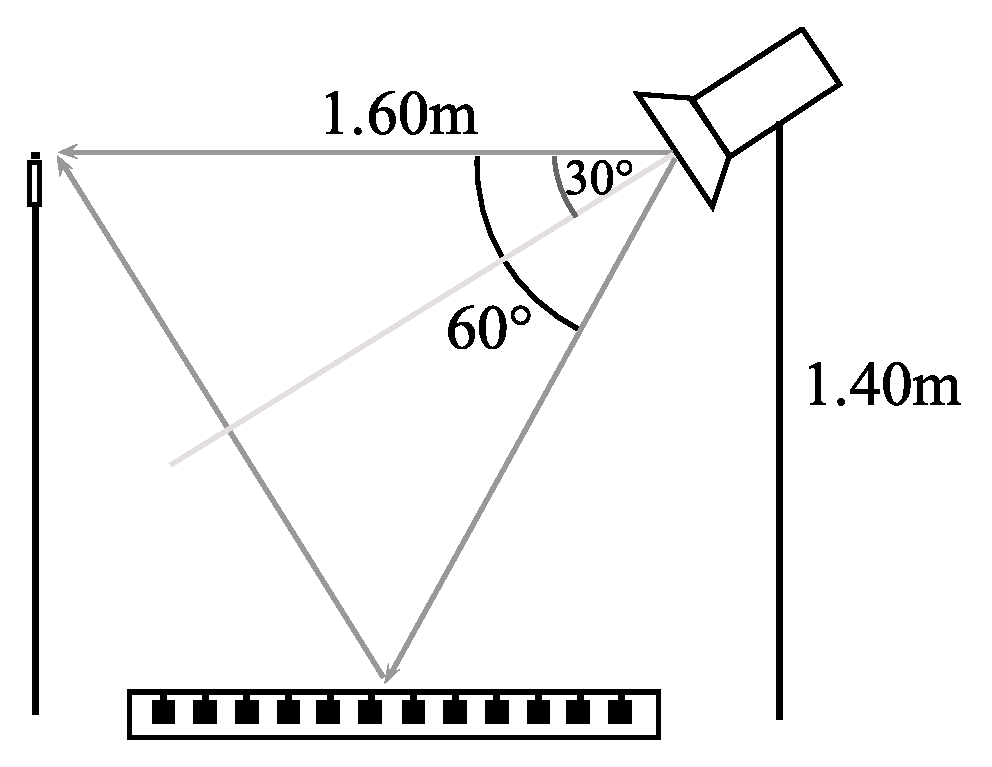
\includegraphics[width=0.3\textwidth]{helmh}
  \caption{Experimental setup for the measurement of the characteristics of the Helmholtz resonator panel.}
  \label{fig: helmh}
  \vspace{-20pt}
\end{wrapfigure}
In order to check the consistency of our program, a measurement was performed to determine the (known) absorption characteristics of a Helmholtz resonator panel. The experimental setup is presented in figure \ref{fig: helmh}. The Zircon loudspeaker is positioned at an angle of $30^{\circ}$ with  respect to the horizontal. This is to ensure that both the resonator panel and the microphone receive a similar signal from the speaker.

Figure \ref{helmsub} shows the results of a measurement with a MLS of order 16 as excitation signal which was averaged 64 times. The graph 
 contains the impulse response of the system, the free field impulse response, the subtracted signal and the used Adrienne temporal window. Figure \ref{helmspec} shows the spectrum of the subtracted signal deconvolved with the free field impulse response. The hyperbolic tangent window seen on the same figure was used to determine the impulse response of the Helmholtz resonator panel shown in figure \ref{helmimp}.
 
  

\figOctaveTwo{helm}{Impulse responses of the measurements and frequency response of the Helmholtz resonator panel.}
	{helmsub}{Total (red), free field (green) and subtracted (black) impulse responses and the Adrienne temporal window (blue).}
	{helmspec}{Spectrum of the Helmholtz resonator (blue) and the hyperbolic tangent window (green).}


\begin{figure}[h!]
  \centering
    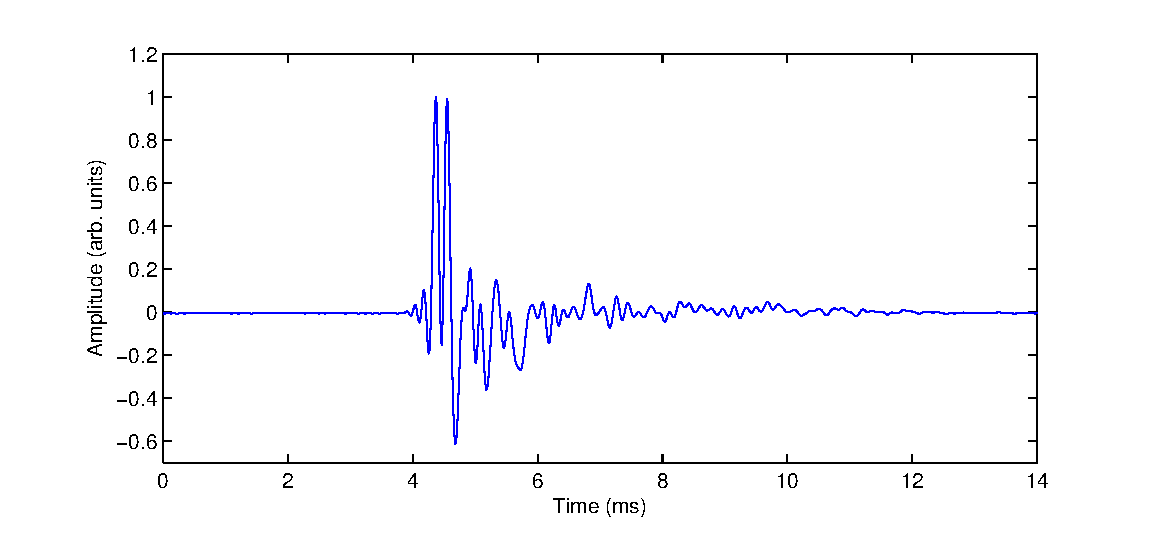
\includegraphics[width=\textwidth]{helmimp}
  %\vspace{-10pt}
  \caption{Impulse response of the Helmholtz resonator panel.}
  \label{fig: helmimp}
  %\vspace{-30pt}
\end{figure}

The frequency dependent absorption coefficient is computed using equation \ref{absorption}. The result of this calculation is displayed in figure \ref{helmalles} as the red line. The other lines represent measurements with other excitation signals: the yellow line is obtained as the average of 16 excitations with an MLS of order 18, the green one with a sweep signal of 60 seconds and the blue line as the average of 64 sweeps of 1 second. It is clear that the results of the various measurements are consistent. Moreover, the results agree more or less with the absorption coefficient determined by L. De Geetere is his PhD thesis \cite[p.84]{Geetere}. 

The main deviations are the extra peak at low frequencies (below 250Hz) in our spectrum and the height of the peak between 6000Hz and 7000Hz. The appearance of the extra peak at low frequencies can be attributed to the effects of windowing in the time domain. The determination of the lowest frequencies will be compromised because of the attenuation at the beginning and tail of the signal. A possible explanation for the peak at 6500Hz being too high lies in the directionality of the Zircon loudspeaker. As can be seen in figure \ref{thetavar}, the spectrum has a sudden decrease in power at frequencies around 6500Hz and at values for $\theta$ between $45\degr$ and $60\degr$. Since the speaker was positioned at $\theta = 120\degr$ in an attempt to give the direct and reflected sound the same speaker response, the angle between speaker and horizontal was \emph{approximately} $30\degr$. It is thus possible that due to a small deviation of the angle, the speaker responses (at 6500Hz) were not exactly the same for both travel paths. The reflected path received less power at 6500Hz from the speaker, which would show in the spectrum of the reflected component as pit, or consequently as a enlarger peak in the absorption coefficient.


\begin{figure}[h!]
  \centering
    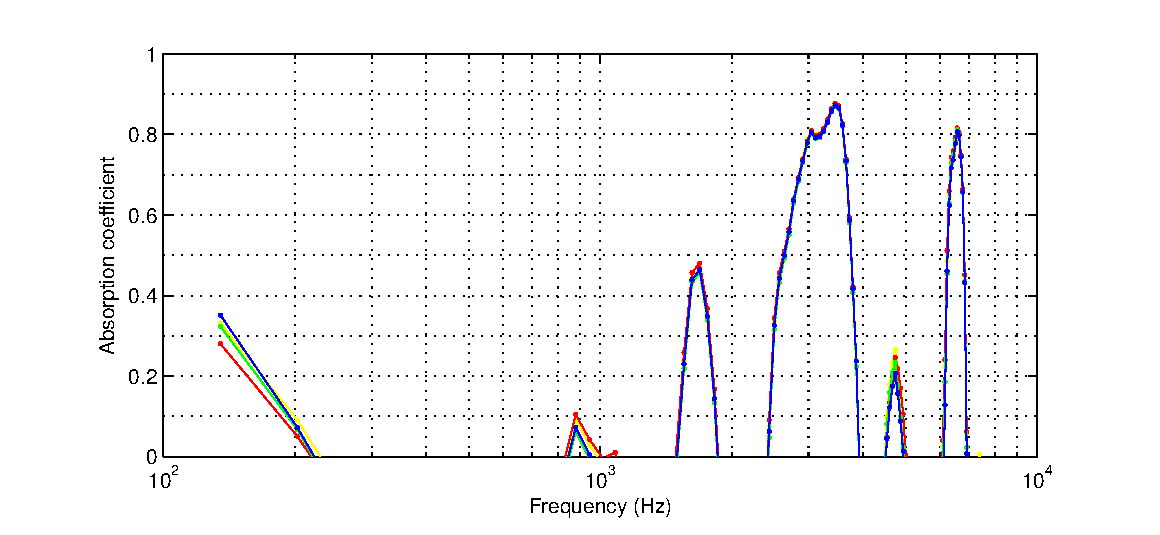
\includegraphics[width=\textwidth]{helmalles}
  %\vspace{-10pt}
  \caption{Absorption coefficient of the Helmholtz resonator determined with different excitation signals: 16$\times$ MLS of order 18 (yellow), 64$\times$ MLS of order 16 (red), 1$\times$ sweep of 60s (green), 64$\times$ sweep of 1s (blue).}
  \label{fig: helmholtzalles}
  %\vspace{-30pt}
\end{figure}


\subsection{The Adrienne method}
The acoustical characterisation of objects is an essential part in the design of noise reducing devices, such as the noise barriers along a motorway. It is important to be able to evaluate the performance of such barriers and more importantly to be able to compare them objectively. In order to do so a series of standardized methods was developed by CEN (European committee for standardization) to determine the performance of such devices. One of these methods determines the sound reflection of the device and is called the Adrienne method. A short description of the Adrienne method and its shortcomings will be given in this section. For more details, see the technical specification CEN/TS 1793-5:2003 \cite{Adrienne}.



\subsubsection{Experimental setup}

\begin{wrapfigure}{r}{0.5\textwidth}
	\vspace{-10pt}
  \centering
    \includegraphics[width=0.48\textwidth]{Adrienne.pdf}
  \caption{Setup for the reflection index measurements according to the Adrienne method.}
  \label{fig: adrienne}
  \vspace{-40pt}
\end{wrapfigure}
The Adrienne method requires the setup shown in figure \ref{fig: adrienne}\footnote{This image was taken from \cite[p.45]{Geetere}.}. The microphone is attached to the speaker, such that the distance between them is 1.25m. The speaker is placed at a distance of 1.50m of the wall. The speaker and microphone assembly are capable of rotating. A set of nine measurement is performed with the angle varying between $50\degr$ and $130\degr$ in steps of $10\degr$.  Several sets of measurement have to be executed at different positions and rotating along different axes dependent on the homogeneity of the sample.
The excitation signal is a MLS and the signal is averaged at least 16 times.


\subsubsection{Data processing}\label{adrwindow}
The processing of the data happens as follows: the impulse response of a measurement is determined using cross correlation. The reflected component is extracted from the total impulse response by subtracting the direct component (obtained from a free field measurement). A time window is placed on the reflected component to remove parasitic reflections (for example from the floor). The window selected for this purpose is called the Adrienne temporal window and it has the following specifications \cite{Adrienne}:
\vspace{-20pt}
\begin{itemize}
	\setlength{\itemsep}{1pt}
  \setlength{\parskip}{0pt}
  \setlength{\parsep}{0pt}
	\item a leading edge of 0.5 ms with a left-half Blackman-Harris shape,
	\item a flat portion of length 5.18 ms,
	\item a trailing edge of 2.22 ms with a right-half Blackman-Harris shape.
\end{itemize}
\vspace{-20pt}
The full Blackman-Harris window of length T is defined as 
\[
w(t) = 0.35875 - 0.48829 \cos(\frac{2 \pi t}{T}) + 0.14128 \cos(\frac{4 \pi t}{T}) - 0.01168 \cos(\frac{6 \pi t}{T}).
\]
This window shall be placed such that its flat portion begins 0.2 ms before the first peak of the needed impulse response.

With these ingredients a parameter called the reflection index of the device under test is computed in 1/3 octave bands using the following formula 
\[
RI_j = \frac{1}{n_j} \sum^{n_j}_{k=1} \frac{\int_{\Delta f_j} \left|\mathcal{F}\left[t\cdot h_{r,k}(t)\cdot w_r(t)\right]\right|^2 \,df }{\int_{\Delta f_j} \left|\mathcal{F}\left[t \cdot h_{i}(t) \cdot w_i(t)\right]\right|^2 \,df }
\]
with \\

\begin{tabular}{ll}
$h_i(t)$ & the free field impulse response \\
$h_{r,k}(t) = h_k(t) - h_i(t)$ & the reflected component of the impulse response at the k-th angle \\
$w_i(t)$ & the Adrienne window for the free field impulse response\\ 
$w_r(t)$ & the Adrienne window for the reflected component of the impulse response\\ 
$\mathcal{F}$ & the symbol for Fourier transform \\
$\Delta f_j$ & the width of the j-th one third octave frequency band\\
$n_j$ & the number of angles on which to average\\ 
\end{tabular}
The parameter $t$ which is added to both the numerator and denominator is 
The reflection index is a measure for the average ratio of reflected energy and incident energy. It is this standardized quantity that is used to compare the reflection capacities of different noise barriers. For more details, see \cite{Adrienne}.

\subsubsection{Shortcomings}
\begin{wrapfigure}{r}{0.5\textwidth}
	\vspace{-10pt}
  \centering
    \includegraphics[width=0.48\textwidth]{adriennedir}
  \caption{Path of the reflected wave.}
  \label{fig: adriennedir}
  \vspace{-40pt}
\end{wrapfigure}
The problem with the Adrienne method is that the directionality of the speaker is not accounted for. For example: when measuring at an angle of $130\degr$, the path of the reflected wave will resemble figure \ref{fig: adriennedir}. It is clear that the reflected component was emitted at a different angle than the direct component. Hence the reflected component contains a different speaker response. And this was only the case for a flat surface, imagine what would happen for non flat walls. Another disadvantage of this setup is that the speaker itself can be the cause of the first parasitic reflection which limits the time window, since it stands relatively close to the wall. Therefore, it would be advisedly to place the speaker at greater distance from the wall and keep the microphone close to it.

This would not only solve the problem of parasitic reflections from the speaker, it would also reduce the influence of the speaker's directivity. The solid angle in which the response of the speaker can be considered as more or less equal remains the same, but the effective surface on the wall becomes larger. The angle between the direct sound path and the reflected sound path becomes smaller as the speaker is further removed of the wall. And hence the influence of the speaker diminishes.

The disadvantage of placing the speaker further away, is that the reflection with the ground comes quicker after the reflected sound. This results in shorter Adrienne windows and consequently a larger lowest frequency limit. The solution to this problem would be to place the speaker and microphone higher. This however results in parasitic reflections due to diffraction effects at the top of the wall.   





\subsection{In situ measurement}
Gebruik de mls measurements, want buiten gemeten en rekening houden met extra artifacten (vandaar windowen)
niet echt praktisch
Octave bands conform the norm. Probleem voor banden bij lage frequenties:
helaas uitstap echte muur afgelast
{\huge Warning: for meaningful design results, center frequency used should preferably be in range Fs/200 < Fc < Fs/5.}

p 68 de geetere heeft ook de muur gemeten!




%\end{document}
